\documentclass[12pt]{article}
\usepackage[utf8]{inputenc}
\usepackage{graphics}
\usepackage{amsmath}
\usepackage{graphicx}
\usepackage{geometry}
\usepackage{caption}
\usepackage{url}
\usepackage{booktabs}
\usepackage{tabularx}
\usepackage{hyperref}
\usepackage{float}
\usepackage{ulem}
\hypersetup{
	colorlinks=true,
	linkcolor=blue,
	filecolor=magenta,      
	urlcolor=cyan,
	pdftitle={Overleaf Example},
	pdfpagemode=FullScreen,
}

\urlstyle{same}



\title{Software Requirements Specification: Chrome Dino Runner \\ \bigskip \large SFWRENG 3XA3 Project \\ \bigskip \large Team Number: L03 Group 1 \\ \large Team Name: ``Team Rex'' }

\author{Chelsea Maramot \\ maramotc \\ \\ Anjola Adewale \\ adewaa1 \\ \\ Sheridan Fong \\ fongs7 }

\date{February 11 2022}

\begin{document}
	
	\maketitle
	\newpage
	\tableofcontents
	% section 1: Project Drivers ---------------------------
	\section{Project Drivers}
	\subsection{The Purpose of the Project}
	The current pandemic has abruptly disrupted the entertainment sector, and now people are seeking entertainment within the comfort of their homes. An example of an at-home entertainment solution is video games. We aim to provide home entertainment by redesigning the classic Chrome T-Rex dinosaur game. We plan to improve its user-friendliness and interactivity while maintaining the game’s basic functionality. The game's development will follow the software development process and be implemented in python using the Pygame library. The entire process will be documented\textcolor{blue}{.} \sout{and tested using the unit test framework.}  \textcolor{blue}{To verify the project we will use manual, dynamic and automated testing approaches.}
	\subsection{The Stakeholders}
	\subsubsection{The Client}
	The clients for this project are the course instructor of SFWRENG 3XA3, Dr. Ashgar Bokhari, and the teaching assistants (TAs), Stephanie Koehl, Veersah Palanichamy and Abdul Rab Mohammed. The clients will provide project requirements, deliverables and deadlines. They will also provide guidance when necessary and evaluate the project with respect to the requirements in the SRS document. 
	\subsubsection{The Customers}
	The customers for this project are individuals who are interested in playing Chrome Dino Runner. The project does not explicitly target a demographic but is rather designed as a general-purpose entertainment source. The project is designed for anyone with the game's required software, which is Python and the Pygame library. 
	\subsubsection{Other Stakeholders}
	All members of group one are the stakeholders of this project. We are all responsible for the development process, such as implementing, testing, and documenting the project. Group one members all care for the project's success and are responsible for maintaining the repository. Developers that fork the repository and continue the project's development are also stakeholders as they will be continuing the project and are interested in the project's success
	
	
	% Section 2: Project Constraints 
	\section{Project Constraints}
	Project constraints are restrictions on the product due to the budget or the 
	time available to build the product.
	\subsection{Mandated Constraints}
	\subsubsection{Solution Design Constraints}
	\textbf{Description:} The game \sout{(an executable file)} must be able to run on any machine running on Windows 7 or newer, macOS 10.12 or newer or Linux Ubuntu  16.04 or newer.
	\\ \\
	\textbf{Rationale:} Most computer users already use systems with these specification and so the users will not need to purchase a new system. \\ \\
	\textbf{Fit Criterion:} The game will be developed into an \sout{executable} file that will be made to run on Windows or newer, macOS Sierra 10.12 or newer or Linux Ubuntu 16.04 or newer.
	\subsubsection{Implementation Environment of the Current System}
	N/A
	\subsubsection{Partner of a Collaborative Application}
	N/A
	\subsubsection{Off-the-Shelf Software}
	N/A
	\subsubsection{Anticipated Workable Environment}
	N/A
	\subsubsection{Schedule Constraints}
	\textbf{Description:} This project must follow the project schedule outlined in the Gantt chart and the Task Section. \\ \\ 
	\textbf{Rationale:} Due to the time constraints on this project(3 months), this project needs to follow
	a predefined plan in order to ensure successful completion. \\ \\ 
	\textbf{Fit Criterion:} All deliverable contained within this project must be completed and submitted by April 12, 2022. 
	
	\subsubsection{Budget Constraints}
	N/A
	
	
	\subsection{Naming Conventions and Terminology}
	See Table ~\ref{table:naming} for Naming Conventions and Terminology
	\begin{table}[] 
		\centering
		\caption{Table of Naming Conventions and Terminology.}
		\begin{tabular}{l c p{.5\textwidth}}
			\toprule
			Term       && Definition \\
			\midrule
			Basic English Proficiency && Knowledge of vocabulary words, ability to speak simple phrases or sentences \\
			\midrule
			Chrome Dino Runner  && The game that will be implemented by Team Rex. \\
			\midrule
			Game play && This refers to the activity of playing the game. \\
			\midrule
			High Score          && Highest score achieved by the player \\
			\midrule
			
			Leaderboard && This refers to the page that display's the high scores of the game and the respective user's name. \\
			\midrule 
			Obstacles && This refers to any objects that the user has to jump over in game play. \\
			\midrule
			Pygame              && A cross-platform set of Python modules designed for writing video games. \\
			\midrule
			Python              && The programming language used in developing Chrome Dino Runner. \\
			\midrule
			
			Settings menu && This refers to the page where user's can change audio and theme settings. \\
			\midrule
			Score               && A numerical value which quantifies the player's performance the game. \\
			\midrule
			SRS       && Acronym for Software Requirements Specification; a document that describes what the system will do and the expected performance. \\
			\midrule
			User       && The Individual who will be playing  our game. \\
			\midrule
			WASD keys           && Four keyboard keys that are used to interact with video games in lieu of Arrow keys or a controller. W and S control forward and backward movement, while A and D are left and right \\
			
			
			\bottomrule
		\end{tabular}
		\label{table:naming}
	\end{table}
	
	\subsection{Relevant Facts and Assumptions}
	\subsubsection{Facts}
	The original repository contains 350 lines of code and is developed in Python using the Pygame library. 
	\subsubsection{Assumptions}
	\begin{itemize}
		\item Users possess a computer running Windows 7 or newer, macOS 10.12 or newer or Linux Ubuntu 16.04 or newer
		\item User have basic English proficiency 
		\item Users know how to operate a PC
		\item Users have the visual and physical capabilities to play the game.
	\end{itemize}
	
	% Section 3: Functional Requirements
	\section{Functional Requirements}
	
	\subsection{The Scope of the Work and the Product}
	
	\subsubsection{The Context of the Work}
	% come back to and insert picture properly 
	\begin{figure}[!ht]
		\centering
		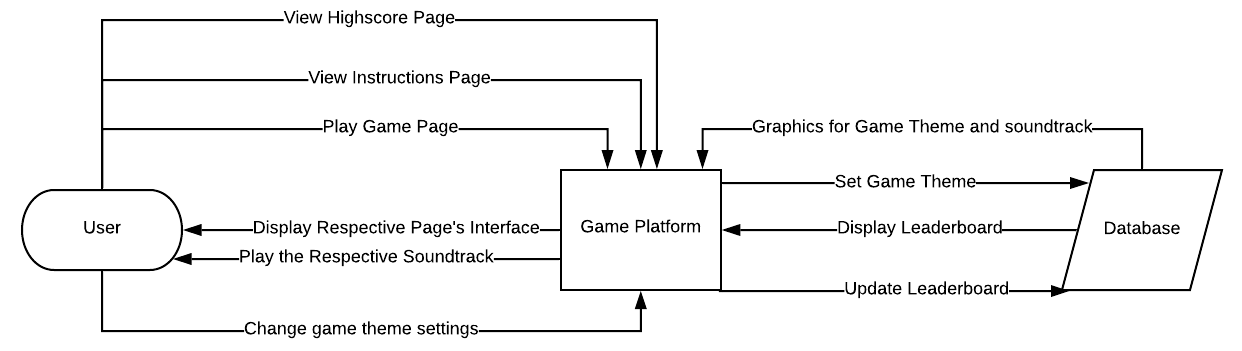
\includegraphics[width=1.02\textwidth]{context_diagram.png}
		\caption{Caption}
	\end{figure}
	
	\subsubsection{Work Partitioning}
	
	
	\noindent\setlength\tabcolsep{4pt}%
	\begin{table}[H]
		\captionof{table}{Work Partitioning Event Details}
		\begin{tabularx}{\linewidth}{|l|c|*{4}{>{\RaggedRight\arraybackslash}X|}}
			\hline
			ID & Event Name & Event Description           & Input                & Expected Output               \\ [0.5ex]
			\hline
			1  & Viewing the Instructions Page  & Displays the instruction page.  & Keyboard/ Mouse  & Instructions page \\
			\hline
			2  & Viewing the Leaderboard  & Displays the leaderboard  & Mouse & Leaderboard page  \\
			\hline
			3  & Change Game Settings  & The user can select different themes for the game, changes will be reflected in the UI. They can also alter the audio output. & Theme name and sound settings & Interface display and audio \\
			\hline
			4  & Playing the Game &The user plays the dino game  & Keyboard/     Mouse & Interface display, theme music and final display \\
			\hline
		\end{tabularx}
	\end{table}
	\vskip1cm
	
	
	
	\subsubsection{Individual Product Use Cases}
	
	\begin{figure}[H]
		\centering
		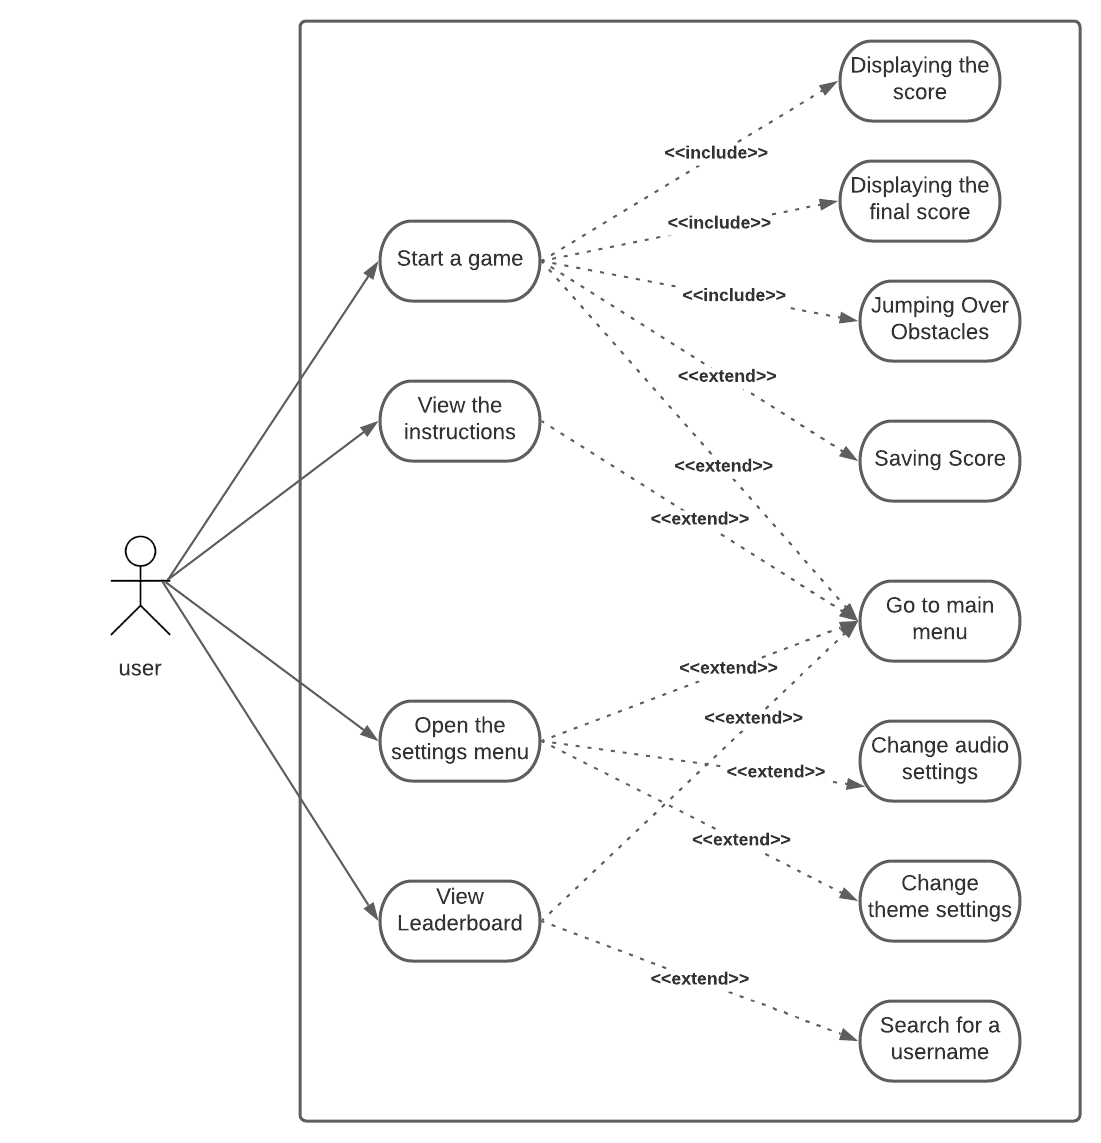
\includegraphics[scale=1.4]{use_case.png}
		\caption{A use case diagram that displays the functionality of the application.}
	\end{figure}
	
	The use case diagram above shows the different ways a user can interact with the system. The user can start a game and the game must include the current score, allow the user to jump over or duck under obstacles and at the end of gameplay display the final score. Game play is not impacted on whether a user goes to the main menu or if the score is saved to the database. Therefore, these action extend the use case. The use cases for viewing the instructions page, leaderboard page and settings menu are all self-explanatory. 
	
	
	
	\subsection{Functional Requirements}
	
	\textbf{E1: Viewing the Instructions Page} \newline
	FR1. The system must display instructions on how to play the game to the user. \newline
	FR2. The system must provide the user with a way to navigate the main menu. \newline \newline
	\textbf{E2: Viewing the Leaderboard} \newline
	FR3. The system must display \sout{ the user with} a list of the players with top scores and the respective score.  \newline
	FR4. The system must provide the user with a way to navigate back to the main menu. \newline
	FR5. The system must be able to filter the high scores \sout{by user}. \newline \newline
	\textbf{E3: Change Game Settings} \newline
	FR6. The system must provide the user with a way to exit from the game settings to the main menu. \newline
	FR7. The system must allow the user to change the audio settings on the game, such as having no audio or audio. \newline
	FR8. The system must display the available themes and allow the user to select a theme. \newline \newline
	\textbf{E4: Playing the Game} \newline
	FR9. The system must display the game to the screen with the appropriate theme. \newline
	FR10. The system must initialize the score to 0 when starting the game. \newline
	FR11. The system must output sound based on the audio settings. \newline
	FR12. The system must start gameplay when the user inputs a \sout{WASD} keyboard command. \newline
	FR13. The system must allow WASD, \textcolor{blue}{arrow and spacebar} keyboard inputs to control the user interface.\newline
	FR14. The system must award points to the user after each dino step. \newline
	FR15. The system must display the user’s current score to the screen. \newline
	FR16. The system must allow the user to replay the game. \newline
	FR17. The system must allow the user to stop the game and return to the main menu. \newline
	FR18. The system must allow the user to enter their username \textcolor{blue}{before they start} \sout{when they are done} playing the game. \newline
	FR19. After the game is finished, the user score must be entered into the database. \newline
	
	
	
	% section 4 -----------------------
	\section{Non-Functional Requirements}
	\subsection{Look and Feel Requirements}
	\subsubsection{Appearance Requirements}
	LF1. The user interface shall consist of essential components relevant to the game.
	\subsubsection{Style Requirements} 
	LF2. The product shall maintain the 90's arcade appearance.\\
	LF3. The product shall incorporate different themes.\\
	LF4. The game colours shall not distract the user's game play.
	
	\subsection{Usability and Humanity Requirements}
	\subsubsection{Ease-Of-Use Requirements}
	UH1. The game shall be controlled using two methods: arrow keys or WASD.\\
	UH2. The game shall have a simple menu page where the game can be accessed easily.\\
	UH3. The game shall be used by people intuitively, no training needed and at a minimum basic English level.
	
	\subsubsection{Personalization and Internationalization Requirements}
	UH4. The product shall only be used in English.\\
	UH5. The user can adjust the theme of the game based on their preferences.
	
	\subsubsection{Learning Requirements}
	UH6. The user shall not require training before playing the game.\\
	UH7. The game must contain basic instructions within the main menu page.
	
	\subsubsection{Understandability and Politeness Requirements}
	UH8. The game shall encompass a level of abstraction from the user.\\
	UH9. The game shall use common control keys to play the game.\\
	UH10. The game will include universal symbols and words that are naturally understood by the user community.
	
	\subsubsection{Accessibility Requirements}
	UH11. The game shall be playable for users with colour blindness.\\
	UH12. The game shall use appropriate font style and size, making it readable to the general public.
	
	\subsection{Performance Requirements}
	\subsubsection{Speed and Latency Requirements}
	PE1. Scores shall be uploaded to the leaderboard in less than 10 seconds after game play.\\
	PE2. The interface must have a maximum response time of 2 seconds to avoid disrupting the user's game play.\\
	PE3. The game shall update the new status parameters within 5 seconds of user input.
	
	\subsubsection{Safety-Critical Requirements}
	N/A
	
	\subsubsection{Precision or Accuracy Requirements}
	PE4. Integer whole number scores shall be uploaded and displayed on the screen within 900 milliseconds of changing.\\
	PE5. The leaderboard shall be updated according to the top integer score.\\
	PE6. The game shall have a maximum latency of 900 milliseconds.
	
	\subsubsection{Reliability and Availability Requirements}
	N/A
	
	\subsubsection{Robustness or Fault-Tolerance Requirements}
	N/A
	
	\subsubsection{Capacity Requirements}
	PE7. The game \textcolor{blue}{when played locally} shall only be available to a single player at a time.\\
	PE8. The game shall allow a maximum of 5 users stored in the leaderboard.
	
	\subsubsection{Scalability or Extensibility Requirements}
	PE9. Developers shall be able to add new features, such as themes, without compromising the basic functionalities of the game. 
	
	\subsubsection{Longevity Requirements}
	PE10. The game shall maintain functionality with existing software until Spring 2022.
	
	\subsection{Operational and Environmental Requirements}
	\subsubsection{Expected Physical Environment}
	PE11. The game shall be played with full functionality without an internet connection.\\
	PE12. The game shall be played within any computer operating system (i.e. Linux, Windows).
	
	\subsection{Requirements for Interfacing with Adjacent Systems}
	\subsubsection{Productization Requirements}
	PE13. The game shall be distributed to user computers as an executable file.\\
	PE14. The game shall be installed without the use of separately printed instructions.
	
	\subsection{Release Requirements}
	PE15. The game shall be released by April 12, 2022.
	
	\subsection{Maintainability and Support Requirements}
	\subsubsection{Maintenance Requirements}
	MA1. Source code shall be updated with the latest changes, within one working week of the scheduled agreement date.\\
	MA2. Source code shall be appropriately documented.
	
	\subsubsection{Supportability Requirements}
	MA3. The full project source code shall be made available to Git users in order to raise issues.
	
	\subsubsection{Adaptability Requirements}
	MA4. The product shall run under Windows 10, macOS Sierra 10.12, Linux Ubuntu 16.04, or newer versions of these operating systems.
	
	\subsection{Security Requirements}
	\subsubsection{Access Requirements}
	SR1. The game users shall have read-only access to the leaderboard and user scores. \\
	SR2. Users are permitted to change game settings through user interface.
	
	\subsubsection{Integrity Requirements}
	SR3. The product shall protect itself from unauthorized user modifications.\\
	SR4. The user shall not be allowed to modify scores.
	
	\subsubsection{Privacy Requirements}
	SR5. Each user shall only be able to view other user names and their corresponding high scores within the leaderboard.
	
	\subsubsection{Audit Requirements}
	N/A
	
	\subsubsection{Immunity Requirements}
	SR6. The product shall not be vulnerable to unauthorized or undesirable software programs.
	
	\subsection{Cultural and Political Requirements}
	\subsubsection{Cultural Requirements}
	CP1. The game themes shall not be offensive to any cultures or religions. \\
	CP2. The game shall not allow users to input offensive English user names or from other languages.
	
	\subsubsection{Political Requirements}    N/A
	
	\subsection{Legal Requirements}
	\subsubsection{Compliance Requirements}
	N/A
	
	\subsubsection{Standards Requirements} 
	N/A
	
	\subsection{Health and Safety Requirements}
	N/A
	
	
	%section 5
	\section{Project Issues}
	\subsection{Open Issues}
	There are currently no open issues in the Chrome Dino Runner repository.
	However, the game developers recommended Pygame version 2.0.1 but we found that the current version 2.1.1 is also compatible with the game.
	In addition, the code writes into a score.txt file that does not exist in the initial code repository. For this reason, we had to manually create and populate the score.txt file to successfully compile and run the game.
	\subsection{Off-the-Shelf Solutions}
	A version of the game we are re-implementing is available on Chrome's offline mode and multiple websites including
	https://chromedino.com/, https://dino-chrome.com/en and more.
	Finally, during the 2021 Olympic Games in Tokyo, Google released
	a limited edition themed version of the Dino game which is no longer available. 
	\subsection{New Problems}
	This new implementation of the game will not change the basic rules of the game.
	Players who are accustomed to the original version of the game should be able to play the our version without
	the need for instructions
	\subsection{Tasks}
	
	Tasks are scheduled and delegated as per the project
	\label{subsec:Tasks}
	\href{https://gitlab.cas.mcmaster.ca/maramotc/se3xa3/-/blob/main/GanttChart.pdf}{\color{blue}Gantt Chart}.
	
	\subsection{Migration to the New Product}
	An updated version of our product will include increased number of themes and additional features. The product will be designed with a focus on usability and entertainment. All of these new features and updates will be updated on the repository and issues/bugs will be fixed on a consistent basis. 
	
	\subsection{Risks}
	This project has minimal risk as it is designed for entertainment purposes. The significant risk of this project will be in terms of testing. The quality of our game will depend on the graphical user interface. Testing GUI’s poses challenges as the only testing method available would be system testing. Compared to unit testing, system testing increases the change of bugs and issues going undiscovered. Our game must also be compatible with different hardware configurations and on multiple operating systems.
	\subsection{Costs}
	This project does not have any costs associated with it as it is being developed with open-source software and resources. The only cost is time resources; these resources will be used for the development, documentation and testing of the project. 
	\subsection{User Documentation and Training}
	\subsubsection{Documentation}
	An instructions page will be available in the main menu of the game.
	This page will contain instructions on how the game is to be played as well as the keys that can be used as controls. Information regarding scoring will also be present in this page.
	Finally, the main repository of the game will include a README file, which will detail the installation and set-up instructions.
	\subsubsection{Training}
	A user can play the \textbf{Chrome Dino Runner} with no necessary training. The game's controls (WASD and arrows) should be intuitive when jumping over obstacles. The player may practice the game to improve skill, but no prior training is needed to succeed.  
	\subsection{Waiting Room}
	% ## do we just put our improvements here?? I think so - SF
	\begin{itemize}
		\item Adding background music to the game to match the speed of the dinosaur
		\item Developing a themed version of the game 
		\begin{itemize}
			\item For example: McMaster student theme, Covid-19 theme
		\end{itemize}
		\item Inserting a play again button
		\item Creating additional pages such as a home, leaderboard and  instruction page 
		\item Implementing new button control and keyboard binding such as A,W,S,D keys
		\item Changing module design and incorporating software engineering principles
	\end{itemize}
	\subsection{Ideas for Solutions}
	N/A
\end{document}
